O menino Araújo, filho de biólogos, sempre foi fascinado pelas espécies de cobras que eram criadas no cativeiro da casa.
 Hoje pela manhã ele ganhou um dominó no bingo da escola e, já em casa, formulou o jogo ``A Maior Cobra Legal de Dominós''.
Um jogo de dominó com valores de $0$ até $N$ é composto por todos os pares de inteiros $(i,j)$ que satisfazem $0 \leq i \leq j \leq N$,
uma peça pode ser rotacionada para gerar a peça $(j, i)$, duas peças $(i,j)$ e $(k, \ell)$ se encaixam como $(i,j)(k,l)$ se e somente se $j = k$,
uma sequência de encaixes é uma cobra se cada peça se encaixa a no máximo duas outras peças, uma em cada ponta.
O objetivo do jogo de nosso jovem protagonista é bem simples: formar a maior cobra de dominós usando.
 Por exemplo, se seu jogo de dominó tem peças com valores de $0$ até 3, uma possível maior cobra de se formar teria 9 peças com a seguinte configuração:

\begin{center}
  $( 0,0 )( 0,1 )( 1,1 )( 1,2 )( 2,2 )( 2,0 )( 0,3 )( 3,3 )( 3,1 )$
\end{center}

Observe que a peça 2-3 (ou 3-2, a peça é a mesma) não foi possível de ser usada.
Por outro lado, se o valor de uma lado de suas peças vai até 4, uma possível maior cobra de se formar teria 15 peças com a seguinte configuração:

\begin{center}
 $( 0,0 )( 0,1 )( 1,1 )( 1,2 )( 2,2 )( 2,0 )( 0,3 )( 3,3 )( 3,1 )( 1,4 )( 4,4 )( 4,2 )( 2,3 )( 3,4 )( 4,0 )$
\end{center}

Curioso que é, o menino Araújo solicitou a ajuda dos programadores da Maratona Mineira para criar um programa com a seguinte missão: dado o valor máximo que pode aparecer em uma peça de dominó, informe qual é o tamanho da maior cobra legal de dominós.


\begin{center}
  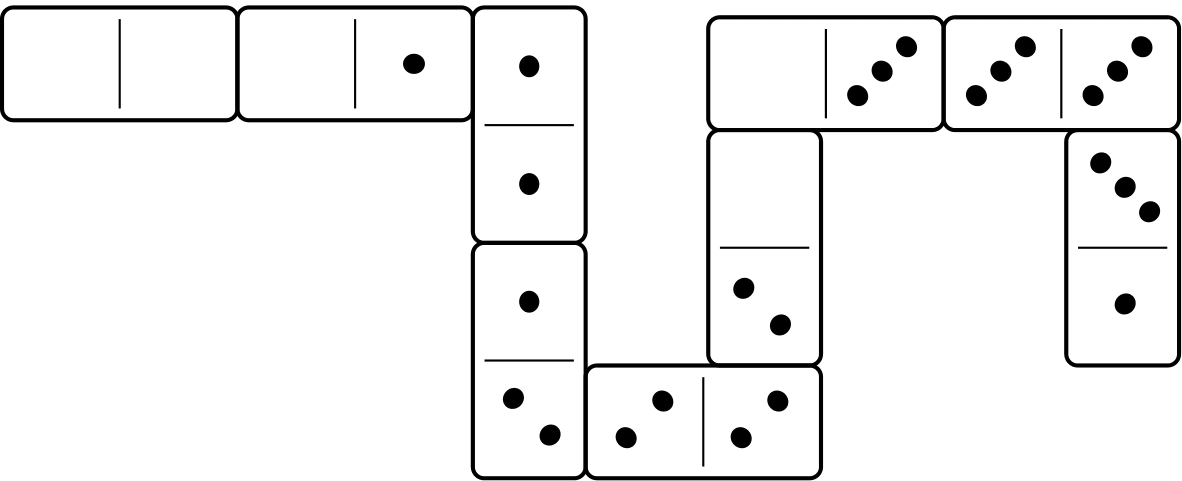
\includegraphics[width=0.7\linewidth]{\CWD/dominos.png}
\end{center}


\section*{Entrada}

A entrada consiste de um único inteiro $N$, o valor máximo que pode existir em uma peça de dominó.


\section*{Saída}

Seu programa deve imprimir um único inteiro, o tamanho da maior cobra de dominó que pode ser formada.


\section*{Restrições}

$$0 \leq N \leq 5000$$

\section*{Exemplos}

\exemplo
